\section{Entrada y salida}

Un módulo de E/S no es únicamente un conector mecánico que permite enchufar el dispositivo al bus del sistema; sino que además está dotado de cierta <<inteligencia>>, que contiene la lógica necesaria para permitir la comunicación entre el periférico y el bus.

Las razones por las que los periféricos no se conectan directamente al bus del sistema son:

\begin{itemize}
  \item Hay una amplia variedad de periféricos con formas de funcionamiento diferentes. Podría ser imposible incorporar la lógica necesaria dentro del procesador para controlar tal diversidad de dispositivos.
  \item Generalmente, la velocidad de transferencia de datos de los periféricos es mucho menor que la de la memoria o el procesador.
  \item Por otro lado, la velocidad de transferencia de algunos periféricos es mayor que la de la memoria o el procesador.
  \item Los periféricos suelen utilizar datos con formatos y tamaños de palabra diferentes de los del computador a los que se conectan.
\end{itemize}

En consecuencia, se necesita un módulo de E/S. Este módulo tiene dos funciones principales:

\begin{itemize}
  \item Realizar la interfaz entre el procesador, la memoria y los periféricos.
  \item Realizar la interfaz entre uno o más dispositivos periféricos.
\end{itemize}

\subsection{Dispositivos externos}

Un dispositivo externo se conecta al computador mediante un enlace a un módulo de E/S. El enlace se utiliza para intercambiar señales de control, estado, y datos entre el módulo de E/S y el dispositivo externo. Los dispositivos externos pueden ser:

\begin{itemize}
  \item \textbf{E/S básicos}: monitor, mouse, teclado, etc.
  \item \textbf{E/S de almacenamiento}: discos duros, CD-ROM, etc.
  \item \textbf{Impresión}: impresoras, escáneres, etc.
  \item \textbf{Comunicaciones}: modems, acceso/interfaz de red, etc.
  \item \textbf{Multimedia}: micrófonos, altavoces, etc.
  \item \textbf{Automatización y control}: sensores, alarmas, etc.
\end{itemize}

\begin{figure}[H]
  \centering
  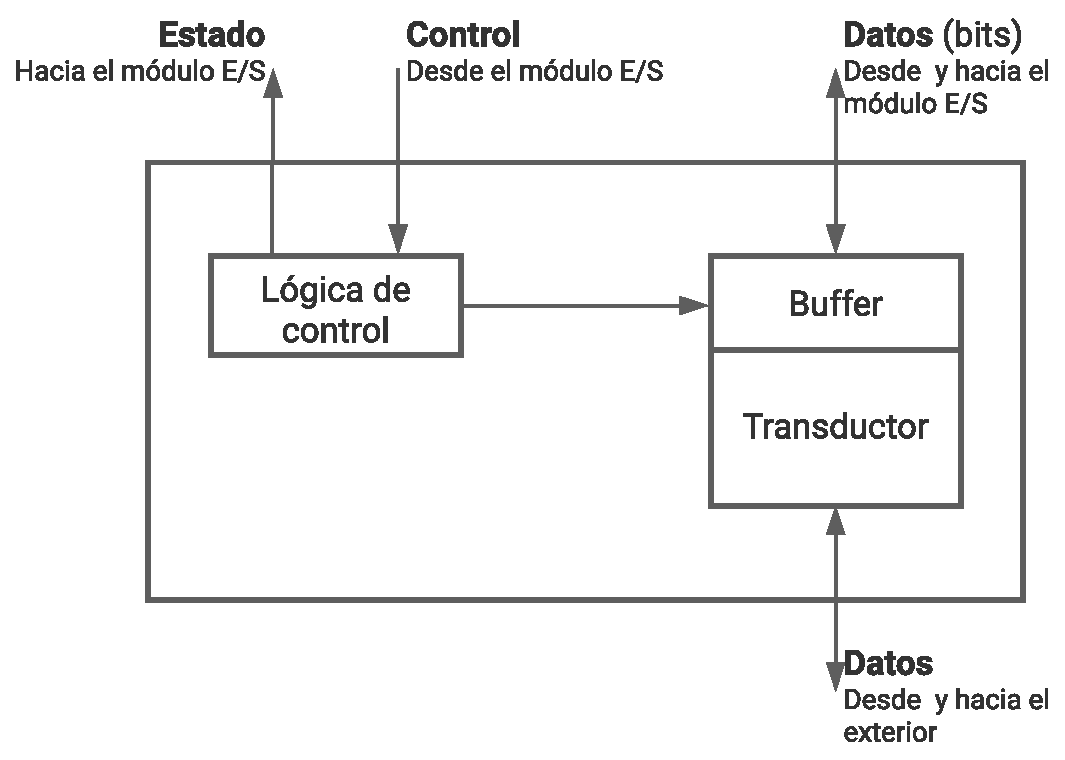
\includegraphics[width=0.6\textwidth]{Dispositivo-externo-tipo}
  \caption{Dispositivo externo}\label{fig:Dispositivo-externo-tipo}
\end{figure}

La forma de un dispositivo externo se indica en la Figura~\ref{fig:Dispositivo-externo-tipo}. La conexión con el módulo de E/S se realiza a través de señales de control, estado y datos.

La \textit{lógica de control} asociada al dispositivo controla su operación en respuesta a las indicaciones del módulo de E/S. El \textit{transductor} convierte las señales eléctricas asociadas al dato a otra forma de energía en el caso de una salida y viceversa en el caso de unta entrada. Existe un buffer asociado al transductor para almacenar temporalmente el dato que se esta transfiriendo entre el módulo de E/S y el exterior.

\subsection{Funciones de un módulo de E/S}

Las principales funciones y requisitos de un módulo de E/S se encuentran dentro de las siguientes categorías:

\begin{itemize}
  \item \textbf{Control y temporización}: coordina el tráfico entre los recursos internos y los dispositivos externos.
  \item \textbf{Comunicación con el procesador}: implica la decodificación de órdenes, el intercambio de datos, información del Estado y el reconocimiento de direcciones.
  \item \textbf{Comunicación con los dispositivos}: esta comunicación implica intercambiar órdenes, información del estado y datos.
  \item \textbf{Almacenamiento temporal de datos}: los datos que se transfieren entre el módulo de E/S y los dispositivos externos se almacenan temporalmente en un buffer.
  \item \textbf{Detección de errores}: detecta los errores e informa al procesador.
\end{itemize}

La complejidad de los módulos de E/S y el número de dispositivos externos que controlan varían considerablemente.

El funcionamiento de un módulo de E/S permite que el procesador vea a una amplia gama de dispositivos de forma simplificada. El módulo debe ocultar los detalles de temporización, formatos y electromecánica de los dispositivos externos para que el procesador pueda funcionar únicamente en términos de órdenes de lectura y escritura.

Un módulo de E/S que se encarga de la mayoría de los detalles del procesamiento, presentando al procesador una interfaz de alto nivel, se denomina \textit{canal de E/S} o \textit{procesador de E/S}. Un módulo que sea bastante simple y requiera control detallado normalmente se denomina \textit{controlador de E/S}.

\begin{figure}[h]
  \centering
  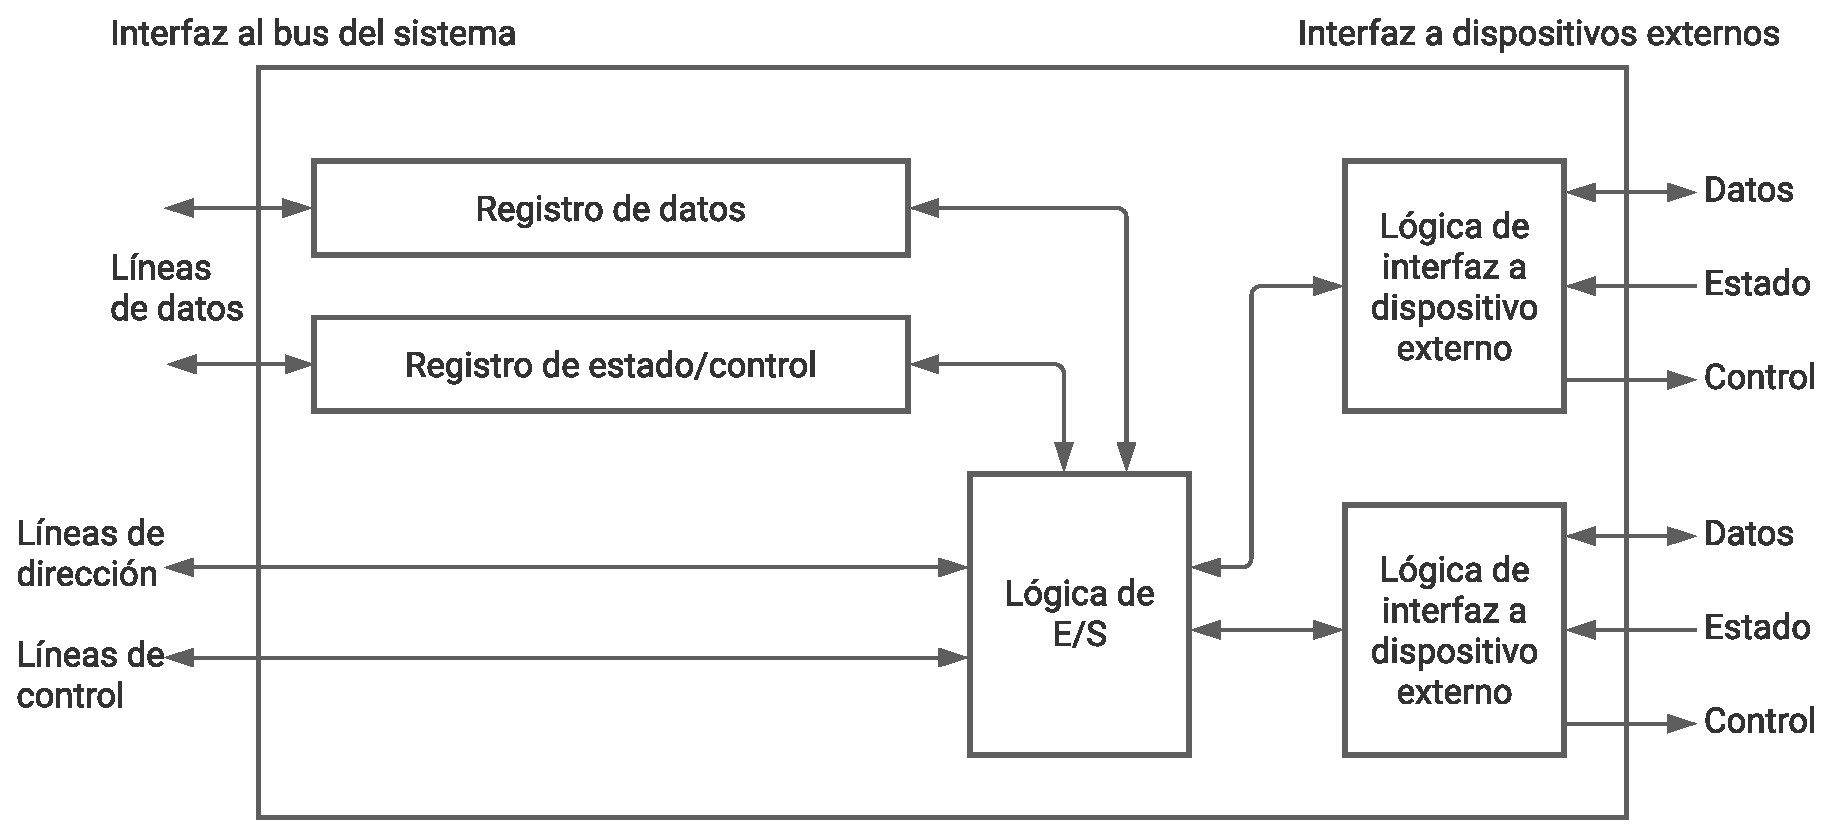
\includegraphics[width=0.6\textwidth]{Modulo-IO}
  \caption{Estructura de un módulo de E/S}\label{fig:Estructura-modulo-E/S}
\end{figure}

\subsection{Entrada y salida programada}

Los datos se intercambian entre el procesador y el módulo de E/S. El procesador ejecuta un programa que controla directamente la operación de E/S:\@
\begin{itemize}
  \item Comprobación del estado del dispositivo.
  \item Envío de una orden de lectura o escritura.
  \item Transferencia del dato.
\end{itemize}

El procesador espera que el módulo de E/S termine la operación.

Los detalles de la E/S programada se muestran en la Figura~\ref{fig:E/S-programada}:

\begin{itemize}
  \item La CPU solicita la operación de E/S.
  \item El módulo E/S realiza la operación.
  \item El módulo E/S activa los bits de estado del dispositivo direccionado y espera.
  \item La CPU comprueba periódicamente el estado de esos bits, hasta que detecta que la operación fue completada.
  \item En caso contrario la CPU espera y vuelve a comprobarlo más tarde.
\end{itemize}

\begin{figure}[h]
  \centering
  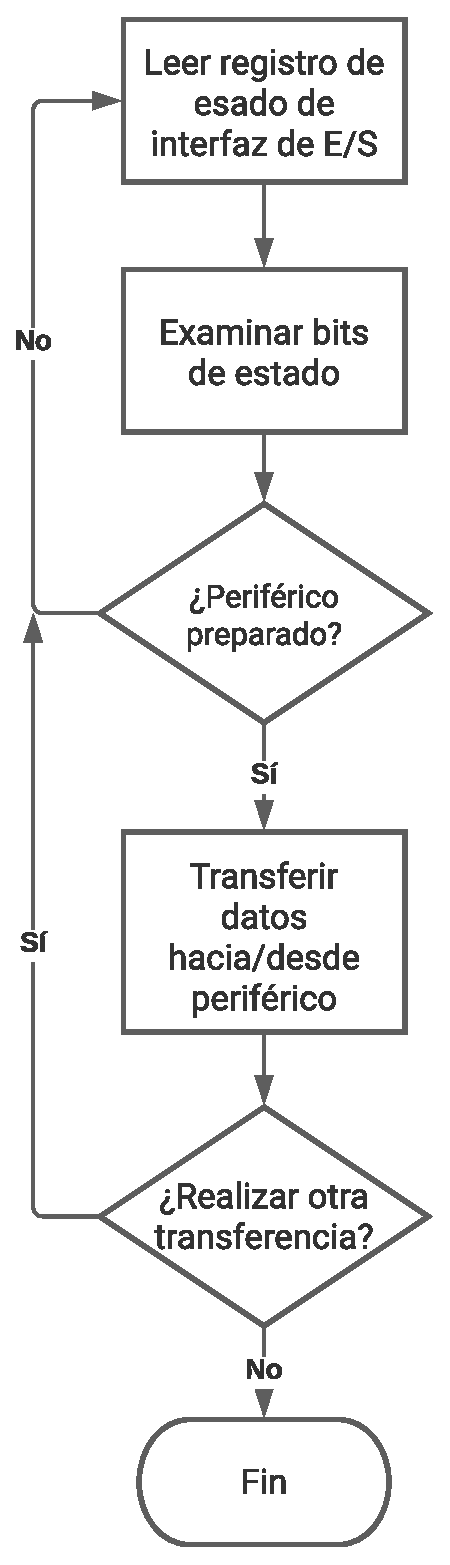
\includegraphics[height=0.38\textheight]{IO-programada}
  \caption{E/S programada}\label{fig:E/S-programada}
\end{figure}

\begin{subs}

  \subsubsection{Órdenes de E/S}
  Al ejecutar una instrucción relacionada con una E/S, el procesador proporciona una dirección, especificando el módulo de E/S particular y el dispositivo externo, y una orden de E/S. Hay cuatro tipos de órdenes de E/S que puede recibir un módulo de E/S cuando es direccionado por el procesador:

  \begin{itemize}
    \item \textbf{Control}: se utiliza para activar el periférico e indicarle qué hacer. Estas órdenes son específicas del tipo particular de periférico.
    \item \textbf{Test}: se utiliza para comprobar diversas condiciones de estado asociadas con el módulo de E/S y sus periféricos.
    \item \textbf{Lectura}: hace que el módulo de E/S capte un dato de un periférico y lo sitúe en un buffer interno. Después el procesador puede obtener el dato solicitando que el módulo de E/S lo ponga en el bus de datos.
    \item \textbf{Escritura}: hace que el módulo de E/S capte un dato del bus de datos y posteriormente lo transmita al periférico.
  \end{itemize}

\end{subs}

\subsection{Entrada y salida con interrupciones}

El problema con la E/S programada es que el procesador tiene que esperar un tiempo considerable a que el módulo de E/S en cuestión esté preparado para recibir o transmitir los datos.

En la E/S con interrupciones, el módulo de E/S interrumpirá al procesador para solicitar su servicio cuando esté preparado para intercambiar datos con él.


Desde el punto de vista del procesador, las acciones son las que siguen:

\begin{itemize}
  \item Envía una orden READ de lectura. El módulo E/S obtiene los datos del periférico mientras la CPU realiza otro trabajo.
  \item La CPU chequea si hay pedidos de interrupciones pendientes al final de cada ciclo de instrucción.
  \item La CPU detecta el pedido, guarda el contexto, interrumpe el proceso y realiza la gestión de la interrupción.
  \item La CPU solicita los datos. El módulo E/S transfiere los datos.
\end{itemize}

\begin{subs}
  \subsubsection{Cuestiones de diseño}

  En la implementación de las E/S mediante interrupciones aparecen dos cuestiones. Primero, cómo determina el procesador qué dispositivo ha provocado la interrupción. Y segundo, si se han producido varias interrupciones, como decide el procesador la que debe atender.

  Hay cuatro tipos de técnicas que se utilizan comúnmente:

  \begin{itemize}
    \item \textbf{Múltiples líneas de interrupción}: consiste en proporcionar varias líneas de interrupción entre el procesador y los módulos de E/S. No resulta práctico dedicar más de unas pocas líneas del bus o terminales del procesador a ser líneas de interrupción.
    \item \textbf{Software poll}: cuando el procesador detecta una interrupción, se produce una bifurcación a una rutina de servicio de interrupción que se encarga de consultar cada módulo de E/S para determinar cuál ha provocado la interrupción. Este método es muy lento y no es muy eficiente.
    \item \textbf{Daisy chain}: es una alternativa a la técnica anterior. Todos los módulos de E/S comparten una línea común para solicitar interrupciones. La línea de reconocimiento de interrupción se conecta encadenando los módulos uno tras otro. Cuando el procesador recibe una interrupción, activa el reconocimiento de interrupción. Esta señal se propaga a través de la secuencia de módulos de E/S hasta que se alcanza un módulo que solicitó la interrupción. El módulo responderá colocando un vector, en el bus, que lo identifica. La CPU emplea el vector como puntero para acceder a la rutina de servicio.
    \item \textbf{Arbitraje de bus}: un módulo de E/S debe en primer lugar disponer del control del bus antes de poder activar la línea de petición de interrupción. Así, solo un módulo puede activar la línea en un mismo instante. Cuando el procesador detecta la interrupción, responde mediante la línea de reconocimiento de interrupción. Después, el módulo que solicitó la interrupción sitúa su vector en las líneas de datos.
  \end{itemize}
\end{subs}

\subsection{Acceso directo a memoria}

El DMA requiere un módulo adicional en el bus del sistema. El módulo o controlador de DMA es capaz de imitar al procesador y de recibir el control del sistema cedido por el procesador. El módulo de DMA utiliza sólo cuando el procesador no lo necesita, o debe forzar al procesador a que suspenda temporalmente su funcionamiento. Esta última técnica es la más común y se denomina \textit{robo de ciclo}.

Cuando el procesador desea leer o escribir un bloque de datos, envía una orden al módulo de DMA, incluyendo la siguiente información:

\begin{itemize}
  \item Si se solicita una lectura o una escritura, utilizando la línea de control de lectura o escritura el procesador y el módulo de DMA.\@
  \item La dirección del dispositivo de E/S en cuestión, indicada a través de las líneas de datos.
  \item La posición inicial de memoria a partir de donde se lee o se escribe indicada a través de las líneas de datos y almacenada por el módulo de DMA en su registro de direcciones.
  \item El número de palabras a leer o escribir, también indicando a través de las líneas de datos y almacenado en el registro de cuenta de datos.
\end{itemize}

El procesador delega la operación de E/S al módulo de DMA, que se encargará de ella. El módulo de DMA transfiere el bloque completo de datos, directamente desde o hacia la memoria, sin que tenga que pasar a través del procesador. Una vez que la transferencia termina, el módulo de DMA envía una señal de interrupción al procesador.

Para una transferencia de E/S de varias palabras, el DMA es mucho más eficiente que la E/S mediante interrupciones o la E/S programada.

Aunque la transferencia por DMA puede ser más eficientes, puede haber ciertos problemas. Se puede degradar el rendimiento de la CPU si el DMA hace uso intensivo del bus.

El problema se reduce con el uso de memoria cache. La mayor parte del tiempo, la CPU lee instrucciones de la cache por lo que no necesita usar el bus de memoria. El DMA puede aprovechar estos intervalos en los que la CPU está leyendo instrucciones de la cache para realizar las transferencias.

En caso de computadores sin cache, el procesador no utiliza el bus en todas las fases de la ejecución de una instrucción. El DMA puede aprovechar las fases de ejecución de una instrucción en las que la CPU no utiliza el bus para realizar sus transferencias.

Si el DMA sólo toma el control del bus durante los intervalos de tiempo en los que la CPU no hace uso del mismo el rendimiento del sistema no sufrirá degradación alguna

Si pueden distinguir dos tipos de transferencias:

\begin{itemize}
  \item Por ráfagas
  \item Por robo de ciclo
\end{itemize}

\begin{subs}
  \subsubsection{DMA modo ráfaga}

  Cuando la CPU concede el bus, el DMA no lo libera hasta haber finalizado la transferencia de todo el bloque de datos completo. La ventaja que tiene es que la transferencia se realiza de forma rápida. Pero la desventaja es que durante el tiempo que dura la transferencia la CPU no puede utilizar el bus con memoria, lo que puede degradar el rendimiento del sistema.

  \subsubsection{DMA modo robo de ciclo}

  Cuando la CPU concede el bus al DMA, se realiza la transferencia de una única palabra y después el DMA libera el bus. El DMA solicita el control del bus tantas veces como sea necesario hasta finalizar la transferencia del bloque completo.

  La ventaja que tiene es que no se degrada el rendimiento del sistema. Aunque por contraparte, la transferencia tarda más tiempo en llevarse a cabo.

  Para la CPU no es considerado una interrupción, por lo que no es necesario guardar el contexto. Si bien el trabajo de la CPU es lento, no será tanto como si ella realizara la transferencia. Por lo tanto, para transferencia de E/S de múltiples palabras, es la técnica más eficiente.

\end{subs}

\subsection{Canales de E/S}

A medida que los computadores han evolucionado, la complejidad y sofisticación de sus componentes se ha incrementado. En ningún lugar se hace más evidente que en el funcionamiento de las E/S. Sus etapas pueden resumirse como:

\begin{enumerate}
  \item La CPU controla directamente los periféricos.
  \item Se agrega un módulo de E/S o controlador.
  \item Idem 2, más llamado de interrupción.
  \item El módulo de E/S provee el acceso directo a memoria (DMA).
  \item El módulo de E/S tiene su propio procesador con su pequeño conjunto de instrucciones.
  \item El módulo además tiene su memoria local, (se convierte en una computadora en sí mismo).
\end{enumerate}

\subsection*{Características de los canales de E/S}

El canal de E/S representa una ampliación del concepto de DMA.\@ Un canal de E/S puede ejecutar instrucciones E/S, lo que le confiere un control completo sobre las operaciones de E/S.

La CPU no ejecuta instrucciones de E/S, sino que los canales toman control completo sobre la transferencia de datos. Las instrucciones de E/S se encuentran almacenadas en la memoria principal para ser ejecutadas por un procesador de uso específico contenido en el propio canal de E/S.

La CPU inicia una transferencia de E/S indicando al canal de E/S que debe ejecutar un programa en la memoria. El programa especifica el dispositivo, el área de memoria para almacenamiento la prioridad y las acciones a realizar en ciertas situaciones de error.

Son comunes dos tipos de canales:

\begin{itemize}
  \item \textbf{Canal selector}: controla varios dispositivos de alta velocidad y se dedica a transferir datos a uno de esos dispositivos. El canal de E/S selecciona un dispositivo y efectúa la transferencia de datos. Los dispositivos son manejados por un controlador o módulo de E/S. Por lo tanto, el canal de E/S ocupa el lugar de la CPU en el control de esos controladores.
  \item \textbf{Canal multiplexor}: puede manejar las E/S de varios dispositivos al mismo tiempo. Para dispositivos de velocidad reducida, un \textit{multiplexor de byte} acepta o transmite caracteres tan rápido como es posible a varios dispositivos. Para dispositivos de velocidad elevada, un \textit{multiplexor de bloque} entrelaza bloques de datos de los distintos dispositivos.
\end{itemize}